\chapter{Experimental}
\label{chap4}

\section{Dual RISC-V Cores in lockstep}
\label{sec:dualcore}

The proposed dual-core architecture is quite straight forward to implement. All that is needed is to connect two cores with synchronization registers at appropriate intervals. Choosing the correct granularity for comparisons is however important. At the highest level, comparing only the output of both cores is an option. Comparison would then have to be done in the \textit{write-back} stage of the pipeline. For the end-user application, this would be the most natural way to do it as the details of what has glitched is far less important than just detecting an error. However, for analyzing the effects of glitch attacks on a system in more detail, a much more fine grained approach is needed. The obvious counterpart to only comparing the output would be to compare all wires and registers. This would allow the user to determine the exact location of an error, but at the cost of adding a lot of hardware. This way of implementing the comparisons can also be argued against as it goes against one of the principal ideas of using a dual-core lockstep mechanism: simplicity of integration. 

As the purpose of this project is to analyze the effectiveness of the dual-core lockstep mechanism, some granularity is needed. However, knowing exactly which wire or register bit has glitched will not be necessary, and adds a lot of extra work for simply connecting everything. Therefore, synchronization registers where comparison happens will be connected to the input signals going to different stages of the pipeline. From this data it is then possible to detect a glitch and give the user some information about exactly where in the pipeline the fault occurred. The top level block diagram for the dual-core lockstep setup is seen in \autoref{fig:dual_block}. As an added security measure, the two cores should be intentionally offset from each other by a few clock cycles. This way, in the unlikely event that an attacker manages to glitch the two cores in precisely the same way at the same time, they now need to do it in a highly synchronized manner, which significantly increases the complexity of the attack. The deliberate offset between the cores introduces a form of time diversity, making it more challenging for an attacker to exploit vulnerabilities using clock glitches or other timing-based attacks. These additional security measures enhance the system's resistance to fault injection attacks and improve its overall robustness.

\begin{figure}[h!]
    \centering
    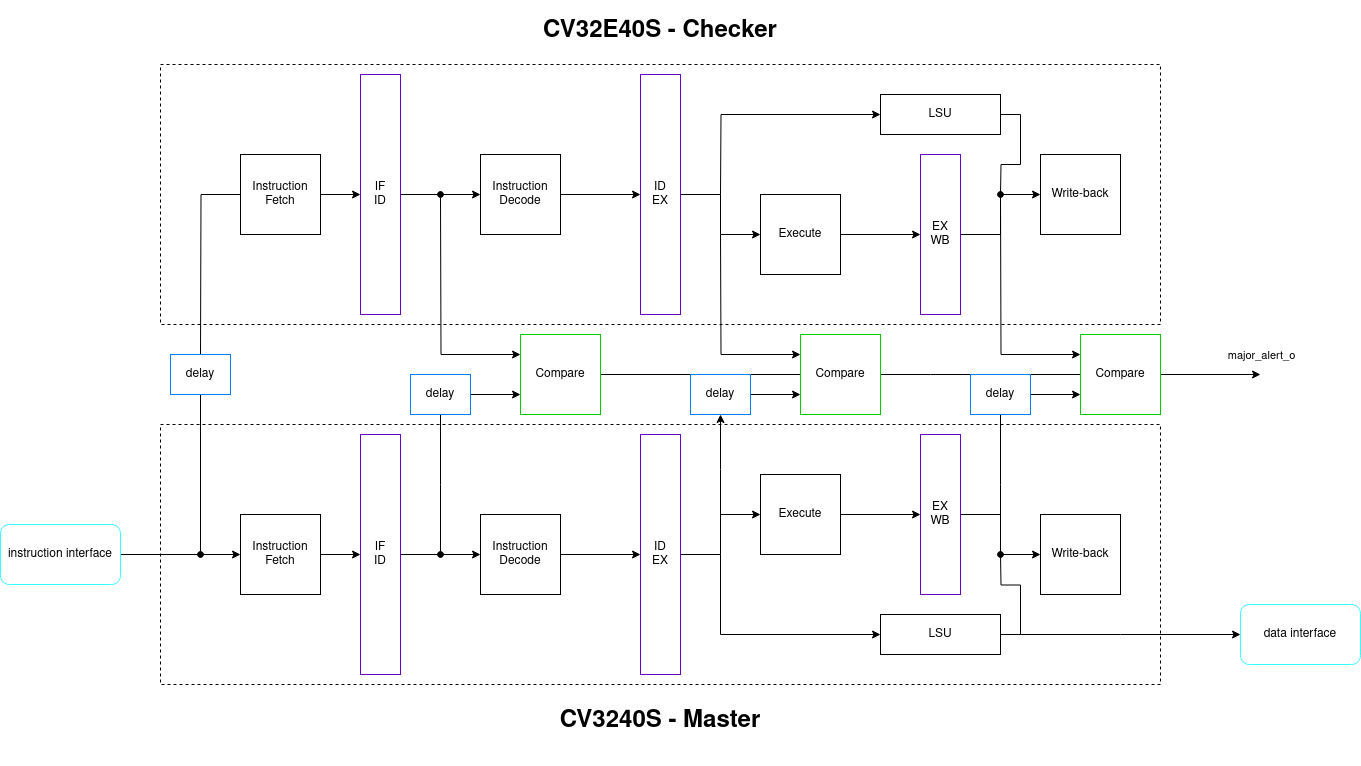
\includegraphics[width=\textwidth]{docs/images/dual_cores_block.png}
    \caption{Block diagram cv32e40s dual-core lockstep mechanism.}
    \label{fig:dual_block}
\end{figure}

\section{Methodology and theory}
\label{sec:method}

\subsection{How are the different layouts tested?}
\subsubsection{Synthesis tool - Which one is used?}
\subsubsection{How is fault injection done in sumlation?}
\subsection{How are results from fault injection compared between the different setups?}

\section{Limitations}
\label{sec:limit}

\section{Choices / Findings}
\label{sec:choice}